\documentclass[conference]{IEEEtran}

\usepackage[utf8]{inputenc}
\usepackage[T1]{fontenc}
\usepackage[spanish]{babel}
\shorthandoff{.<>"}
\usepackage{graphicx}
\usepackage{booktabs}
\usepackage{amsmath}
\usepackage{array}
\usepackage{listings}
\usepackage{xcolor}
\usepackage{tikz}
\usetikzlibrary{positioning,arrows.meta}
\usepackage{cite}

\graphicspath{{../../../figures/}}

\definecolor{azulUSM}{RGB}{0,58,122}

\lstdefinestyle{pseudo}{
    basicstyle=\ttfamily\scriptsize,
    keywordstyle=\bfseries\color{azulUSM},
    commentstyle=\itshape\color{gray},
    morekeywords={mientras,si,sino,retorna,funcion,fin,agendar,encolar},
    breaklines=true,
    frame=single,
    framerule=0.3pt,
    backgroundcolor=\color{black!4},
    xleftmargin=4pt,
    xrightmargin=4pt,
    showstringspaces=false,
}

\AtBeginDocument{%
  \setlength{\abovecaptionskip}{6pt}
  \setlength{\belowcaptionskip}{8pt}
}

\begin{document}

\title{Simulador XG-PON1: Cumplimiento de SLA bajo IPACT, GIANT y QoSDBA}

\author{
\IEEEauthorblockN{David Retuerto, José Vega, Matías Perelli}
\IEEEauthorblockA{
Equipo OmneTeam\\
TEL-341 Simulación de Redes\\
Universidad Técnica Federico Santa María, San Joaquín, Chile\\
\textit{david.retuerto@usm.cl, jose.vargasv@usm.cl, matias.perelli@usm.cl}
}
}

\maketitle

\begin{abstract}
Este trabajo presenta un simulador de eventos discretos, desarrollado en
Python puro sin frameworks externos, para evaluar algoritmos de Asignación
Dinámica de Ancho de Banda (DBA) en una red XG-PON1 (ITU-T G.987) de 8
ONUs. Se comparan IPACT (adaptación de polling de EPON), GIANT (esquema
GPA/SPA nativo de PON) y QoSDBA bajo una tabla de SLA por T-CONT, con foco
en el cumplimiento de latencia de voz (T-CONT1 $\leq$ 2 ms). El modelo se
valida con dos cotas teóricas cerradas (ciclo de polling y latencia
determinista de T-CONT1), que calzan con error menor al 1\% contra los
datos simulados. Los experimentos (9 escenarios $\times$ 10 réplicas,
IC95\%) muestran que GIANT y QoSDBA garantizan 100\% de cumplimiento de
SLA de voz en toda carga probada, mientras IPACT cae a 88.4\% bajo
sobrecarga, a costa de una eficiencia agregada menor en QoSDBA (72.8\%
frente a 94--97\% de IPACT/GIANT).
\end{abstract}

\section{Introducción}

En redes de acceso óptico pasivo (PON), decenas de usuarios comparten una
única fibra y un único canal ascendente. Sin un mecanismo que arbitre el
acceso, servicios con requisitos muy distintos, como una llamada de voz y
una descarga masiva, compiten por el mismo recurso. El algoritmo de
Asignación Dinámica de Ancho de Banda (DBA) que ejecuta la OLT es quien
decide, trama por trama, quién transmite y cuánto.

En el Proyecto 2 de este curso (denominado internamente Fase 2) el equipo
implementó desde cero un simulador de eventos discretos para GPON
(ITU-T G.984), con 32 ONUs y dos algoritmos DBA propios (uno proporcional
y uno con diferenciación de QoS por T-CONT). Tras revisar ese trabajo, la
profesora solicitó un pivote (reunión del 9 de junio de 2026): migrar a
XG-PON1 (ITU-T G.987, el sucesor de 10 Gbps de GPON), reducir a
8 ONUs idénticas, fijar una meta de \emph{Service Level Agreement} (SLA)
explícita para voz ($\leq$ 2 ms) y comparar el DBA propio contra
IPACT, el protocolo de polling de EPON, declarado explícitamente
como referencia de benchmarking y no como mecanismo nativo de PON.

Este informe documenta el simulador resultante (Fase 3 del proyecto), el
modelo de eventos discretos detrás de él, los tres algoritmos DBA
comparados y los resultados experimentales. La Sección \ref{sec:sistema}
describe la red simulada; la Sección \ref{sec:des} detalla el modelo de
simulación de eventos discretos; la Sección \ref{sec:impl} describe la
implementación; la Sección \ref{sec:resultados} presenta la validación
teórica, los experimentos y el análisis estadístico; y la
Sección \ref{sec:conclusiones} cierra con las conclusiones y el trabajo
futuro.

\section{Descripción del Sistema Simulado}
\label{sec:sistema}

\subsection{Red XG-PON1}

XG-PON1 (ITU-T G.987) es el sucesor de 10 Gbps de GPON: mantiene la trama
de control GTC de 125 $\mu$s de G.984.3 pero duplica la tasa ascendente y
cuadruplica la descendente \cite{itu987-1,itu987-2,itu987-3}. La Tabla
\ref{tab:fisicos} resume los parámetros físicos usados, todos derivados
del estándar, sin valores inventados.

\begin{table}[h]
\centering
\caption{Parámetros físicos de la red simulada}
\label{tab:fisicos}
\begin{tabular}{ll}
\toprule
Parámetro & Valor \\
\midrule
Tasa upstream & 2.48832 Gbps \\
Tasa downstream & 9.95328 Gbps \\
Trama GTC & 125 $\mu$s (8000/s) \\
Bytes/trama upstream & 38\,880 B \\
ONUs & 8, idénticas \\
Distancia fibra & 20 km (Clase N1) \\
Delay de propagación & 5 $\mu$s/km (100 $\mu$s one-way) \\
\bottomrule
\end{tabular}
\end{table}

\begin{figure}[h]
\centering
\begin{tikzpicture}[
    box/.style={draw, rounded corners, align=center, minimum height=0.8cm,
                minimum width=1.7cm, fill=azulUSM!8, font=\scriptsize},
    node distance=0.5cm
]
    \node[box] (olt) {OLT};
    \node[box, right=of olt] (split) {Splitter\\1:8};
    \node[box, right=of split] (onu) {8 ONUs};
    \draw[-{Latex[length=2mm]}] (olt) -- node[above, font=\tiny] {20 km} (split);
    \draw[-{Latex[length=2mm]}] (split) -- (onu);
\end{tikzpicture}
\caption{Topología simulada: OLT, splitter pasivo 1:8 y 8 ONUs idénticas.}
\label{fig:topologia}
\end{figure}

\subsection{T-CONTs y tráfico simulado}

El tráfico se clasifica en T-CONTs (Transmission Containers), no en
categorías 5G. Se usan tres tipos, heredados conceptualmente de Fase 2 y
re-escalados $\times 8$ para T-CONT2 (de forma que cada tipo mantenga el
mismo porcentaje de capacidad del enlace que con 32 ONUs). La Tabla
\ref{tab:tconts} resume los parámetros y la Tabla \ref{tab:sla} la meta de
SLA por T-CONT.

\begin{table}[h]
\centering
\caption{T-CONTs simulados}
\label{tab:tconts}
\begin{tabular}{lccc}
\toprule
T-CONT & Distribución & Tasa & Paquete \\
\midrule
1 (VoIP) & CBR & 1 Mbps & 160 B \\
2 (Video) & Poisson & 40 Mbps & 1000 B \\
4 (Datos) & Pareto $\alpha$=1.5 & 200--800 Mbps\footnotemark[1] & 1400 B \\
\bottomrule
\end{tabular}
\footnotetext[1]{Varía según el escenario experimental, Sección
\ref{sec:experimentos}.}
\end{table}

\begin{table}[h]
\centering
\caption{Tabla de SLA por T-CONT}
\label{tab:sla}
\begin{tabular}{lcl}
\toprule
T-CONT & Cota de latencia & Origen \\
\midrule
1 (VoIP) & $\leq$ 2 ms & Pedido explícito de la profesora \\
2 (Video) & $\leq$ 20 ms & Meta razonable del equipo \\
4 (Datos) & $\leq$ 500 ms & Cota laxa, solo referencia \\
\bottomrule
\end{tabular}
\end{table}

\subsection{Supuestos del modelo}

El modelo simplifica deliberadamente varios aspectos para aislar la
variable de interés (el algoritmo DBA): no se modela GEM, ranging, FEC ni
colisión física; los reportes de las ONUs (DBRu) se simplifican a un
diccionario de ocupación por T-CONT en vez del formato binario real; los
paquetes tienen tamaño fijo por T-CONT; y las 8 ONUs son idénticas (misma
distancia, mismas tasas), un requerimiento explícito de esta fase. IPACT
se declara explícitamente como una adaptación de EPON con fines de
comparación, no como un mecanismo que un OLT XG-PON real ejecutaría.

\section{Modelo de Simulación de Eventos Discretos}
\label{sec:des}

\subsection{Estado del sistema}

El estado del sistema en un instante $t$ está dado por la ocupación de
cada buffer T-CONT de cada ONU (bytes encolados), el último reporte
(DBRu) conocido por la OLT de cada ONU y, solo para los algoritmos que
usan contadores, el estado de turno: los contadores de \emph{service
interval} (SImax/SImin) por ONU en GIANT, o el índice de la ONU que está
siendo sondeada en IPACT.

\subsection{Entidades y atributos}

\begin{itemize}
\item \textit{OLT}: tabla de últimos reportes por ONU, número de trama
actual, algoritmo DBA activo.
\item \textit{ONU}: identificador, diccionario de T-CONTs.
\item \textit{TCont}: tipo (1/2/4), buffer FIFO, capacidad máxima,
generador de tráfico asociado, contadores de paquetes/bytes generados y
descartados.
\item \textit{Paquete}: ONU de origen, tipo de T-CONT, tamaño en bytes,
instante de creación (usado para calcular latencia al llegar a la OLT).
\end{itemize}

\subsection{Lista de Eventos Futuros (FEL)}

La Tabla \ref{tab:fel} lista los tipos de evento implementados. Los tres
primeros y los dos últimos son comunes a los tres algoritmos; los
eventos de \texttt{BWMAP}/\texttt{RECV\_BWMAP} (camino broadcast,
usado por GIANT y QoSDBA) y los de \texttt{GATE}/\texttt{POLL\_NEXT}
(camino polling, usado por IPACT) son mutuamente excluyentes: solo un
conjunto se registra según el algoritmo de la corrida.

\begin{table}[h]
\centering
\caption{Tipos de evento del simulador}
\label{tab:fel}
\begin{tabular}{p{3.5cm}p{3.7cm}}
\toprule
Evento & Acción \\
\midrule
\texttt{ONU\_GENERATE\_TRAFFIC} & Encola un paquete nuevo, se reagenda a sí mismo \\
\texttt{OLT\_GENERATE\_BWMAP} & DBA broadcast (GIANT/QoSDBA), cada 125 $\mu$s \\
\texttt{ONU\_RECEIVE\_BWMAP} & ONU transmite según asignación, envía DBRu \\
\texttt{OLT\_SEND\_GATE} / \texttt{OLT\_POLL\_NEXT} & DBA polling (IPACT), una ONU a la vez \\
\texttt{ONU\_RECEIVE\_GATE} & ONU transmite, envía DBRu (camino IPACT) \\
\texttt{OLT\_RECEIVE\_DATA} & Mide latencia, registra entrega \\
\texttt{OLT\_RECEIVE\_REPORT} & Actualiza el reporte (DBRu) de esa ONU \\
\bottomrule
\end{tabular}
\end{table}

\subsection{Condición de término}

Se usa tiempo de simulación fijo $[0, T]$ con $T=10$ s. El primer segundo
(8000 tramas) se descarta como periodo de \emph{warmup}, siguiendo a Law
y Kelton \cite{lawkelton}, para no medir el transitorio de buffers
inicialmente vacíos. Cada uno de los 9 escenarios (Sección
\ref{sec:experimentos}) se ejecuta 10 veces con semillas distintas
(6767--6776) para poder construir intervalos de confianza.

\subsection{Algoritmo de avance de tiempo}

El motor usa avance por evento siguiente (\emph{next-event time
advance}): no hay un reloj que avanza en pasos fijos, sino una cola de
eventos ordenada por tiempo (un min-heap) de la que se extrae siempre el
evento más próximo.

\begin{lstlisting}[style=pseudo]
mientras la cola de eventos no este vacia:
    evento = sacar el evento mas proximo en el tiempo
    si evento.tiempo > tiempo_limite:
        terminar
    reloj_actual = evento.tiempo   # el reloj salta
    handler = handlers[evento.tipo]
    handler(evento)                # puede agendar nuevos eventos
\end{lstlisting}

La generación de tráfico usa \emph{self-scheduling}: cada paquete agenda
la creación del siguiente, según la distribución de su T-CONT (CBR
determinística para voz, Poisson para video, Pareto $\alpha=1.5$ de cola
pesada para datos, siguiendo el carácter auto-similar del tráfico de
Internet \cite{leland94}). La Fig. \ref{fig:traffic} compara la forma de
llegada de las tres distribuciones (normalizadas a la misma tasa media
solo para esta figura): CBR produce intervalos idénticos, Poisson
intervalos aleatorios sin memoria, y Pareto genera las ráfagas
características de cola pesada.

\begin{figure}[h]
\centering
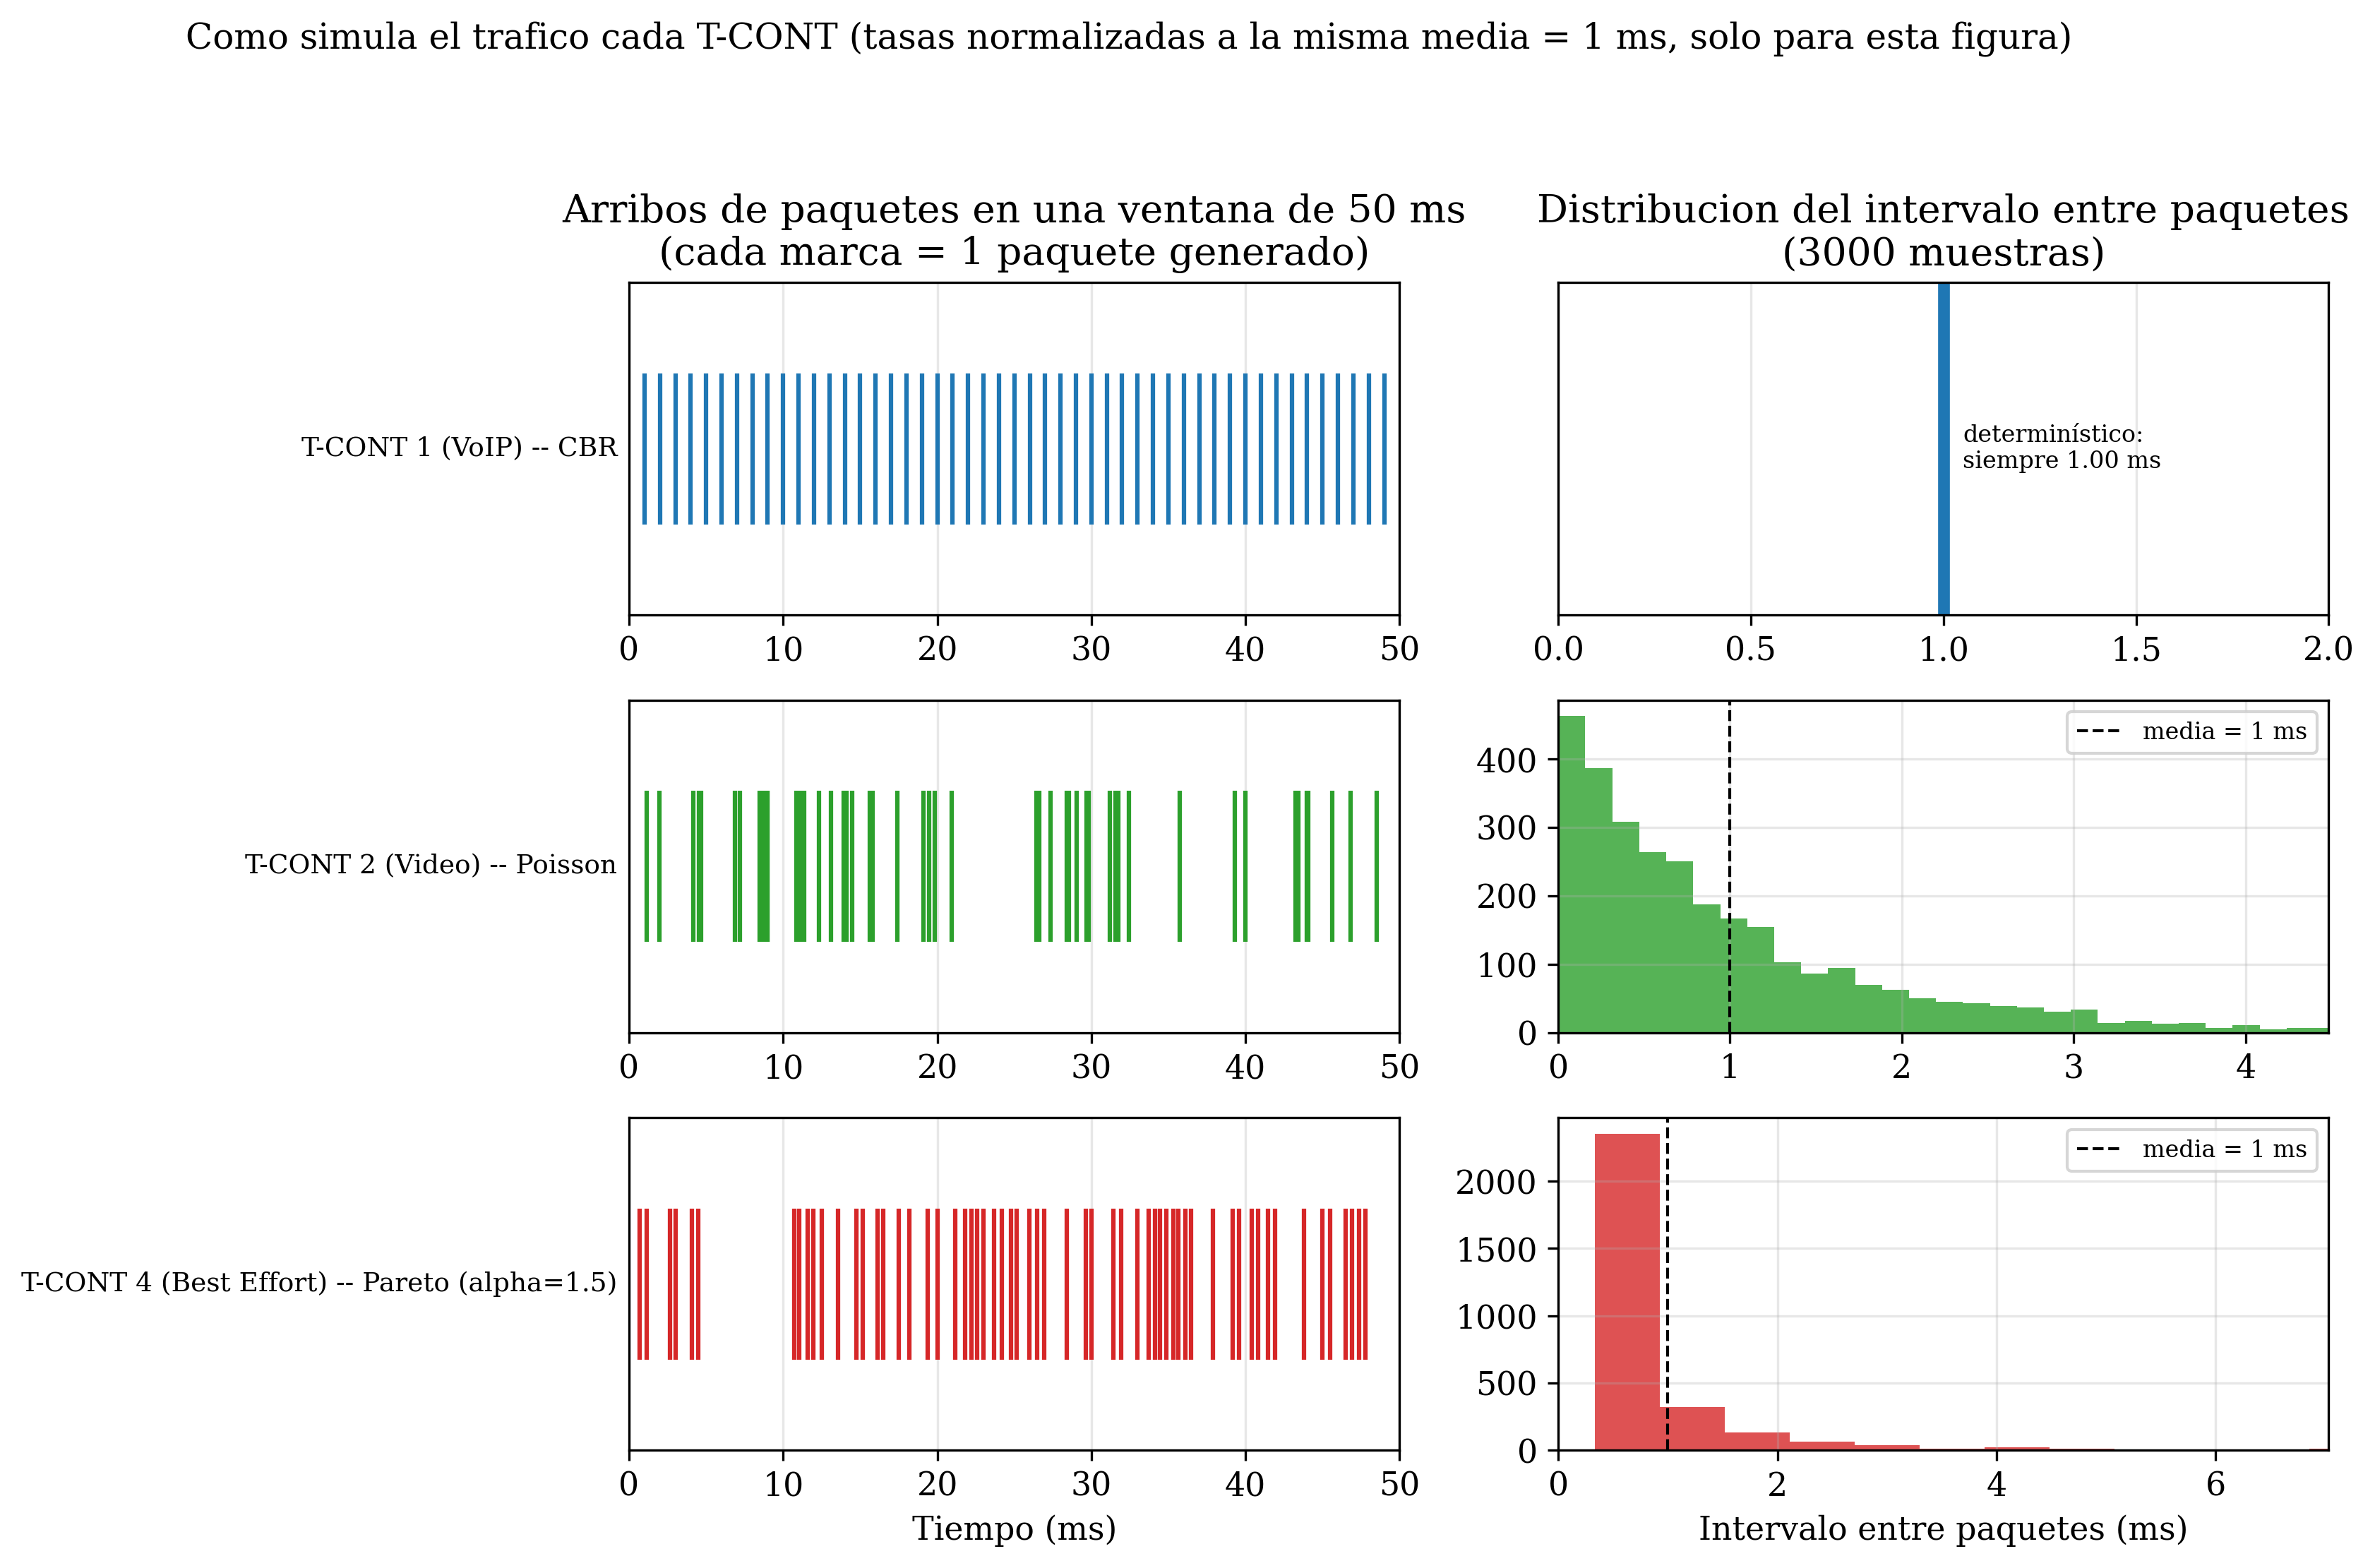
\includegraphics[width=\columnwidth]{traffic_generation.png}
\caption{Llegadas y distribución de intervalos para CBR, Poisson y Pareto.}
\label{fig:traffic}
\end{figure}

\subsection{Entradas del simulador}

Las entradas se dividen en dos clases. Los parámetros físicos
(Tabla \ref{tab:fisicos}) provienen directamente de ITU-T G.987.1/2/3. Los
parámetros de tráfico (tasas de T-CONT2/T-CONT4, contadores
SImax/SImin de GIANT) son decisiones del equipo: T-CONT2 se escaló
$\times 8$ para preservar el mismo porcentaje de capacidad que en Fase 2;
la carga de T-CONT4 se barrió en 200/400/800 Mbps por ONU, preservando las
mismas razones de sobrecarga (64\%/129\%/257\%) usadas en Fase 2; y los
contadores de GIANT (SImax=8, SImin=32 tramas) son una interpretación
propia de la semántica de \emph{service interval} de G.987.3, que el
estándar no fija con un valor único.

\section{Implementación}
\label{sec:impl}

El simulador está escrito en Python 3 puro: el motor de eventos
usa únicamente \texttt{heapq} de la librería estándar, sin SimPy,
OMNeT++ ni ningún otro framework de simulación. El código se organiza en
los módulos de la Tabla \ref{tab:modulos}.

\begin{table}[h]
\centering
\caption{Módulos principales}
\label{tab:modulos}
\footnotesize
\begin{tabular}{p{3.2cm}p{4.0cm}}
\toprule
Módulo & Responsabilidad \\
\midrule
\texttt{engine.py} & Motor DES (heap de eventos, loop principal) \\
\texttt{onu.py}, \texttt{tcont.py} & ONUs, T-CONTs, buffers \\
\texttt{olt.py}, \texttt{olt\_ipact.py} & OLT camino broadcast / polling \\
\texttt{dba\_giant.py} & Algoritmo GIANT \\
\texttt{dba\_ipact.py} & Algoritmo IPACT \\
\texttt{dba\_qos.py} & Algoritmo QoSDBA \\
\texttt{traffic.py} & Generadores CBR/Poisson/Pareto \\
\texttt{metrics/collector.py} & Latencia, SLA, throughput, jitter \\
\texttt{main.py} & CLI de una corrida individual \\
\texttt{run\_experiments.py} & Orquestación de los 9 escenarios \\
\bottomrule
\end{tabular}
\end{table}

Una decisión de diseño central fue mantener Fase 2 (GPON, 32 ONUs)
intacta y construir Fase 3 de forma aditiva: la OLT y la ONU del
camino broadcast (\texttt{olt.py}, \texttt{onu.py}) se reutilizan sin
cambios para GIANT y QoSDBA, mientras que IPACT introduce un camino de
ejecución alternativo y mutuamente excluyente (\texttt{olt\_ipact.py})
que hace polling secuencial round-robin de las 8 ONUs, otorgando a cada
una un grant de servicio limitado: $\text{grant} = \min(\text{demanda
reportada}, B_{max})$, con $B_{max}=38\,880$ B (una trama XG-PON
completa), siguiendo el servicio \emph{limited} de Kramer et al.
\cite{kramer2002}.

GIANT implementa dos fases: GPA (\emph{Guaranteed Phase Allocation},
T-CONT1 fijo e incondicional, T-CONT2 con contador SImax) y SPA
(\emph{Surplus Phase Allocation}, T-CONT4 con contador SImin). Durante
las pruebas de humo se identificaron y corrigieron dos sesgos de equidad
propios de la implementación: (1) sin escalonar el contador de T-CONT2
por ONU, las 8 ONUs competían simultáneamente cada SImax tramas,
sesgando el servicio por orden de iteración; y (2) sin corregir el
puntero \emph{round-robin} de SPA para avanzar solo hasta la última ONU
efectivamente servida, una ONU podía quedar postergada indefinidamente
bajo sobrecarga sostenida. Ambas correcciones son contribuciones propias
del equipo, documentadas como tales.

El Listado \ref{lst:ipact} resume el cálculo del grant de IPACT (servicio
\emph{limited}, aplicado una vez por ONU sondeada) y el Listado
\ref{lst:giant} resume la fase GPA de GIANT para T-CONT2 (contador
SImax escalonado por ONU, con grant de ``catch-up'' cuando el contador
llega a cero).

\begin{lstlisting}[style=pseudo, caption={IPACT: grant por ONU sondeada}, label=lst:ipact]
funcion allocate_onu(onu_id, reporte, B_max):
    demanda_total = suma(reporte.queue_bytes)
    grant_total = min(demanda_total, B_max)
    restante = grant_total
    para tc en [1, 2, 4]:           # prioridad T1>T2>T4
        grant[tc] = min(reporte.queue_bytes[tc], restante)
        restante -= grant[tc]
    retorna grant
\end{lstlisting}

\begin{lstlisting}[style=pseudo, caption={GIANT: fase GPA para T-CONT2 (por trama)}, label=lst:giant]
para cada onu_id:
    si contador_t2[onu_id] == 0:
        cupo = assured_bytes_x_onu * SImax
        grant = min(demanda_t2, cupo, restante)
        bwmap[onu_id][2] = grant
        restante -= grant
        contador_t2[onu_id] = SImax   # reinicia
    sino:
        contador_t2[onu_id] -= 1      # sigue esperando turno
\end{lstlisting}

La Fig. \ref{fig:flow} resume el loop completo del simulador, incluyendo
ambos caminos de ejecución (broadcast a la izquierda, polling a la
derecha) y los cinco bloques de manejo de eventos que se ejecutan en cada
iteración del motor descrito en la Sección \ref{sec:des}.

\begin{figure*}[t]
\centering
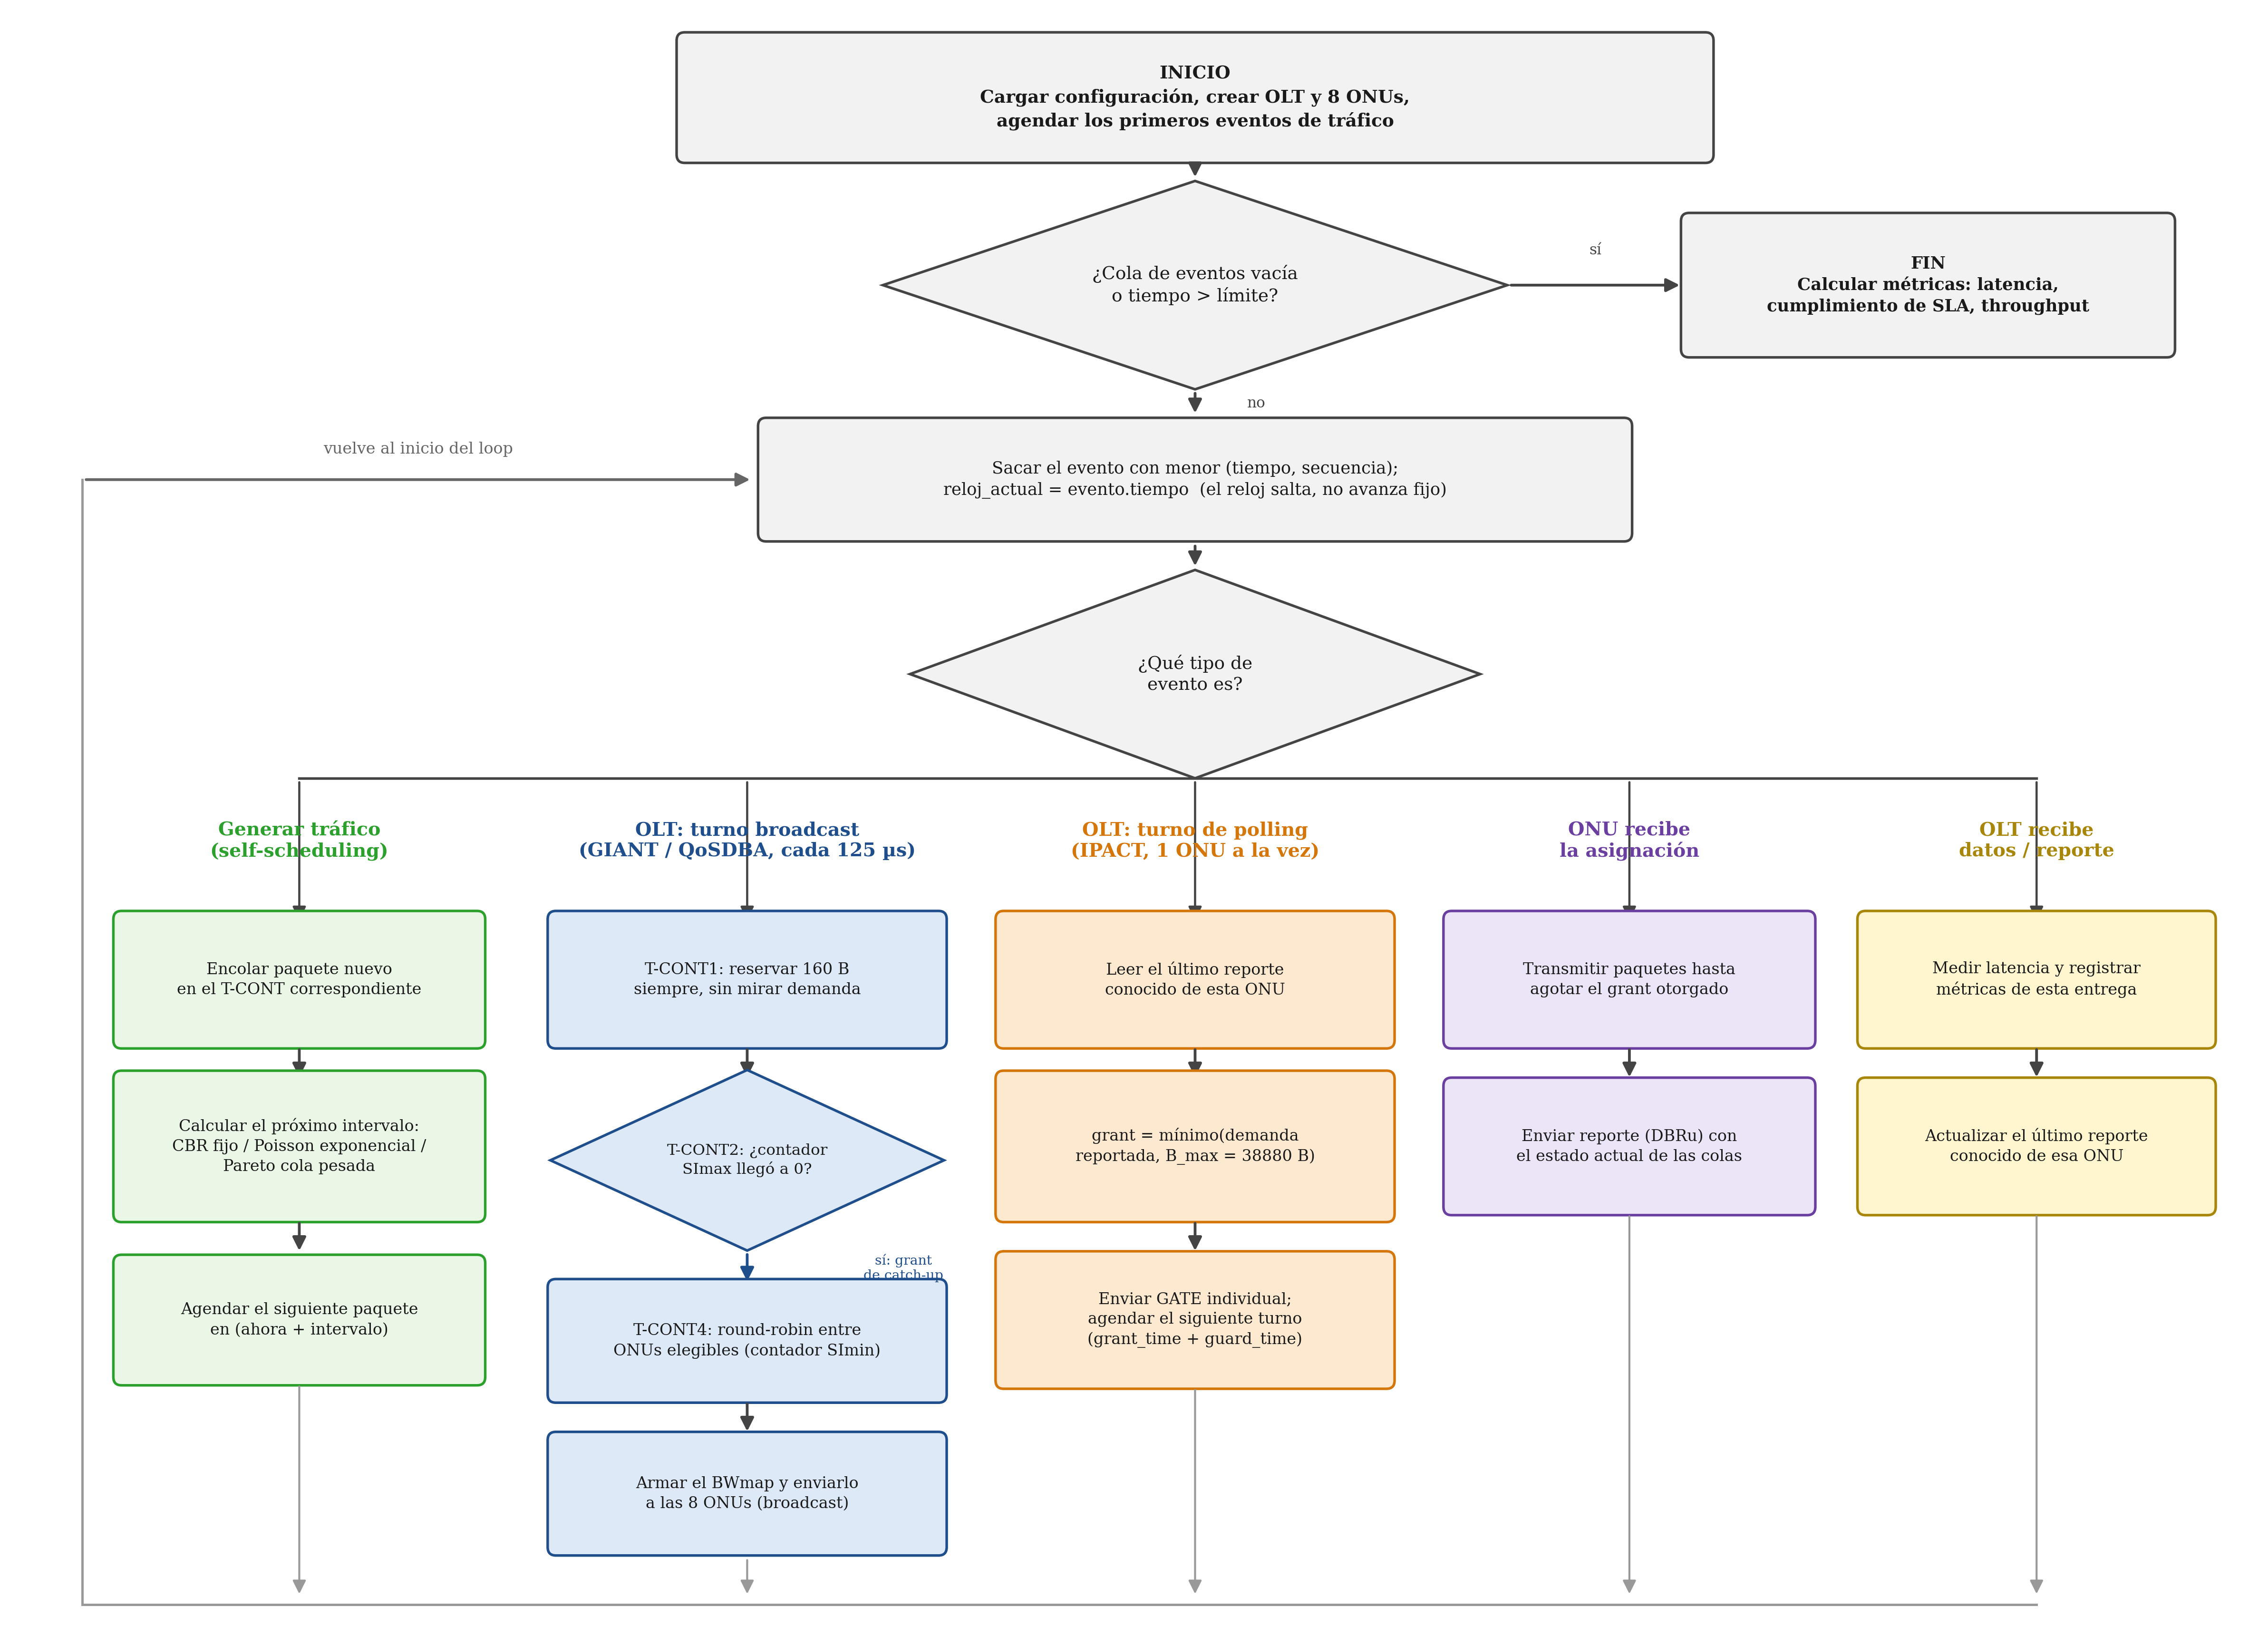
\includegraphics[width=0.92\textwidth]{architecture_diagram.png}
\caption{Diagrama de flujo del simulador: inicialización, extracción del
evento más próximo, y los cinco tipos de manejo de evento (generación de
tráfico, turno broadcast, turno de polling, recepción de asignación, y
recepción de datos/reporte en la OLT).}
\label{fig:flow}
\end{figure*}

\section{Resultados}
\label{sec:resultados}

\subsection{Validación}

El sistema no es una cola M/M/1 clásica, ya que los \emph{grants} son
deterministas o están gobernados por contadores y no por un servidor con
tiempos de servicio exponenciales. Por eso la validación se hace
contrastando dos cotas teóricas cerradas, derivadas directamente del
diseño del algoritmo, contra los datos medidos.

\emph{(a) Ciclo de polling de IPACT.} Con $N=8$ ONUs, tiempo de guarda
$t_{guard}=1\,\mu$s y $B_{max}=38\,880$ B:
\begin{equation}
T_{ciclo} \in \Big[N\,t_{guard},\; N\Big(\frac{8B_{max}}{R}+t_{guard}\Big)\Big]
= [8\,\mu s,\; 1008\,\mu s]
\end{equation}
Bajo saturación (400 y 800 Mbps por ONU) el ciclo medido es exactamente
1008.000 $\mu$s en las 89\,288 y 89\,285 muestras respectivas de
\texttt{cycle\_times.csv}, lo que calza con la cota superior teórica sin
desviación. A carga baja (200 Mbps/ONU) el mínimo medido es 16.23
$\mu$s, por encima del piso teórico de 8 $\mu$s, como se espera porque
ese piso solo se alcanza si las 8 ONUs están simultáneamente vacías.

\emph{(b) Latencia de T-CONT1 bajo GIANT/QoSDBA.} El grant de T-CONT1
(160 B/trama) es fijo e incondicional, y el tráfico es CBR, por lo que la
latencia máxima es una función determinista de la fase entre la llegada
del paquete y la grilla de tramas de 125 $\mu$s:
\begin{equation}
L_{max} = T_{trama} + T_{prop} + T_{tx} = 125 + 100 + 1.03 \approx 226.03\,\mu s
\end{equation}
El valor medido es 226.0288 $\mu$s, con IC95\%=0 en las 10 réplicas, ya
que no hay fuente de aleatoriedad en ese camino, lo que confirma que la
cota es exacta y no una aproximación. La media teórica aproximada
(asumiendo fase uniforme, $\approx 163.5\,\mu$s) también calza con la
medida (164.26 $\mu$s), con un error relativo de 0.44\%.

\subsection{Experimentos}
\label{sec:experimentos}

Se corrieron $3 \times 3 = 9$ escenarios (algoritmo $\in$
\{IPACT, GIANT, QoSDBA\} $\times$ carga de T-CONT4 $\in$
\{200, 400, 800\} Mbps por ONU, equivalentes a 64\%, 129\% y 257\% de
sobrecarga), cada uno con 10 réplicas de 10 s simulados. La Tabla
\ref{tab:resultados} resume los 9 escenarios completos.

\begin{table*}[t]
\centering
\caption{Resultados de los 9 escenarios (media sobre 10 réplicas)}
\label{tab:resultados}
\begin{tabular}{llccccccc}
\toprule
Algoritmo & Carga T4 & \% sobrecarga & SLA T1 (\%) & Lat. máx. T1 ($\mu$s) & SLA T2 (\%) & SLA T4 (\%) & Throughput (Mbps) & Eficiencia (\%) \\
\midrule
IPACT  & 200 Mbps/ONU & 64\%  & 100.00 & 821.21  & 100.00 & 100.00 & 2102.24 & 84.48 \\
IPACT  & 400 Mbps/ONU & 129\% & 88.37  & 2109.08 & 100.00 & 100.00 & 2424.44 & 97.43 \\
IPACT  & 800 Mbps/ONU & 257\% & 88.40  & 2109.05 & 100.00 & 100.00 & 2424.51 & 97.44 \\
GIANT  & 200 Mbps/ONU & 64\%  & 100.00 & 226.03  & 100.00 & 100.00 & 2102.26 & 84.49 \\
GIANT  & 400 Mbps/ONU & 129\% & 100.00 & 226.03  & 100.00 & 100.00 & 2343.30 & 94.17 \\
GIANT  & 800 Mbps/ONU & 257\% & 100.00 & 226.03  & 100.00 & 100.00 & 2343.34 & 94.17 \\
QoSDBA & 200 Mbps/ONU & 64\%  & 100.00 & 226.03  & 100.00 & 100.00 & 1815.86 & 72.98 \\
QoSDBA & 400 Mbps/ONU & 129\% & 100.00 & 226.03  & 100.00 & 100.00 & 1812.82 & 72.85 \\
QoSDBA & 800 Mbps/ONU & 257\% & 100.00 & 226.03  & 100.00 & 100.00 & 1812.62 & 72.85 \\
\bottomrule
\end{tabular}
\end{table*}

Nótese que el cumplimiento de SLA de T-CONT2 y T-CONT4 es 100\% en los 9
escenarios: sus cotas (20 ms y 500 ms respectivamente) son lo bastante
laxas como para no verse comprometidas en el rango de carga probado; el
SLA de T-CONT1 (2 ms) es la única cota que realmente discrimina entre
algoritmos, que es justamente la métrica que la profesora pidió priorizar.

La Fig. \ref{fig:sla} muestra el cumplimiento de SLA por T-CONT: GIANT y
QoSDBA llegan a 100\% en los tres tipos de tráfico en toda carga
probada, mientras IPACT cae a 88.4\% en T-CONT1 (voz) bajo sobrecarga. La
Fig. \ref{fig:delay} muestra por qué: a partir de 400 Mbps por ONU, el
delay máximo de IPACT cruza la cota de SLA de 2 ms, mientras GIANT y
QoSDBA permanecen planos en 226 $\mu$s sin importar la carga. El
mecanismo detrás se ve en la Fig. \ref{fig:cycle}: bajo carga alta el
ciclo de polling de IPACT se vuelve constante en su máximo teórico
(1008 $\mu$s), forzando a T-CONT1 a esperar hasta dos ciclos completos
para ser atendido. El costo de las garantías incondicionales de GIANT y
QoSDBA se observa en la Fig. \ref{fig:throughput}: a 800 Mbps por ONU,
IPACT y GIANT entregan 94--97\% de la capacidad disponible, mientras
QoSDBA se queda en 72.8\% porque su reparto proporcional de T-CONT4 deja
capacidad sin usar.

\begin{figure}[h]
\centering
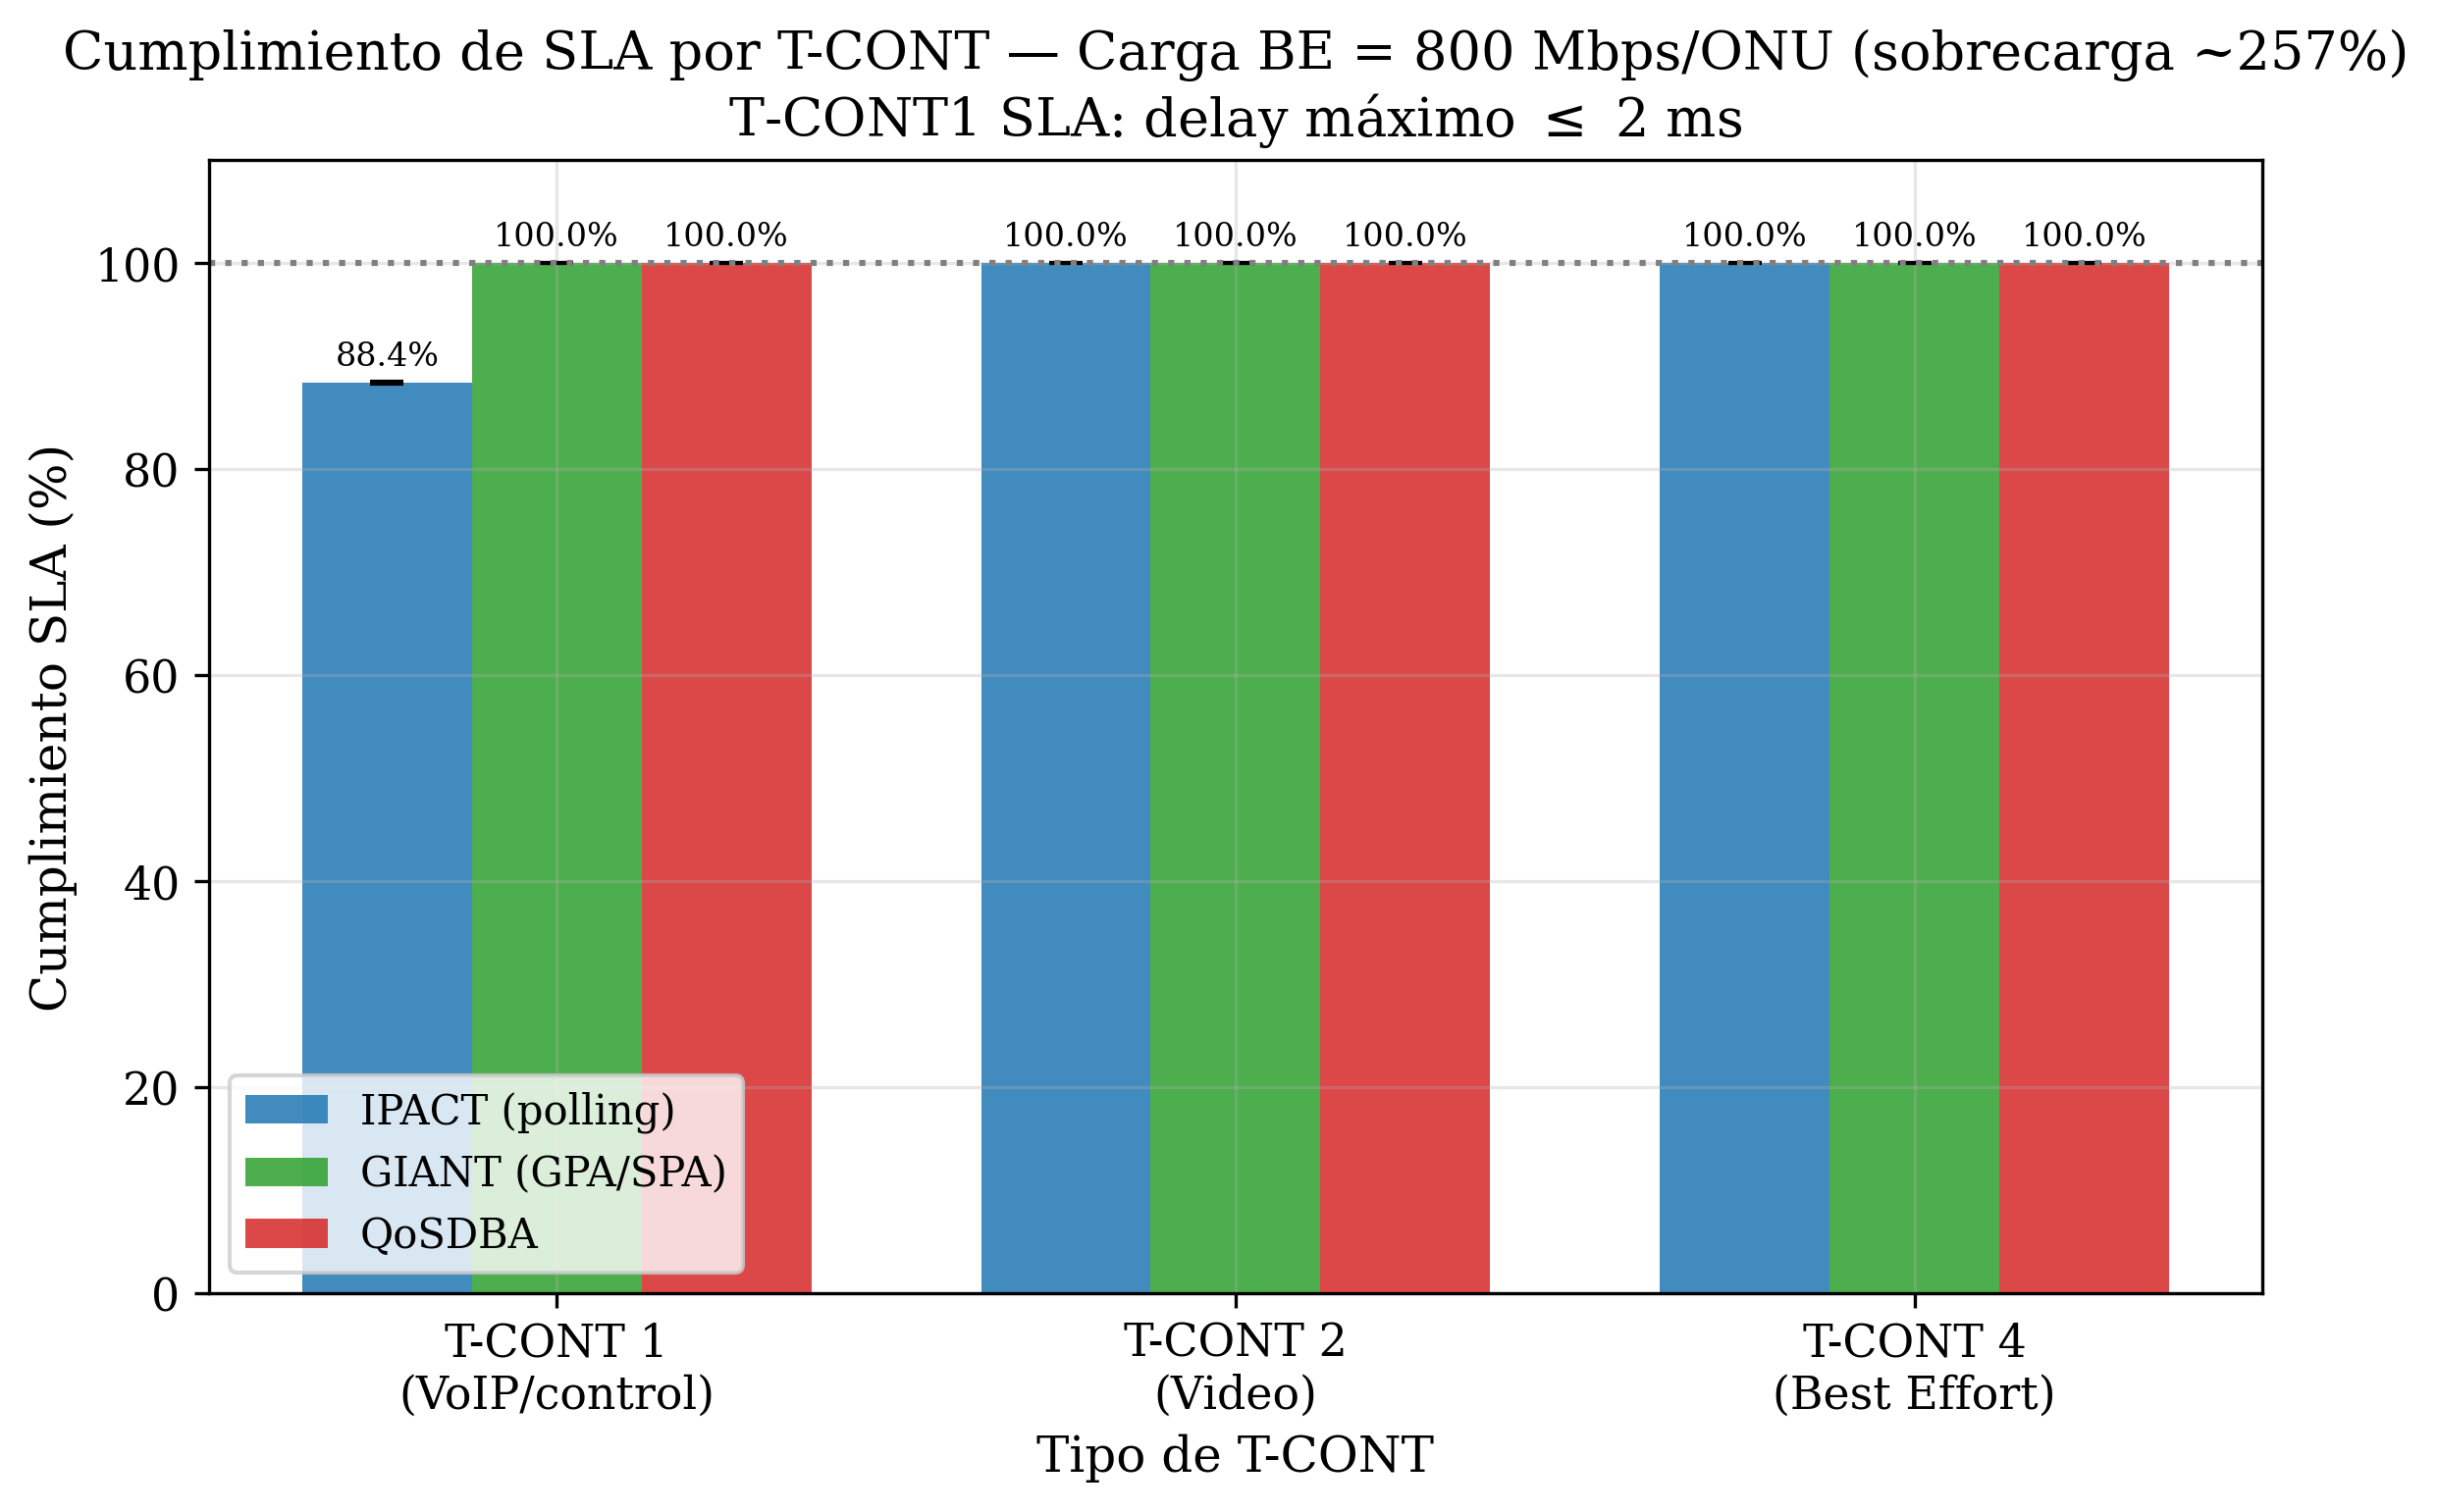
\includegraphics[width=\columnwidth]{sla_compliance_by_tcont.png}
\caption{Cumplimiento de SLA por T-CONT a 800 Mbps/ONU.}
\label{fig:sla}
\end{figure}

\begin{figure}[h]
\centering
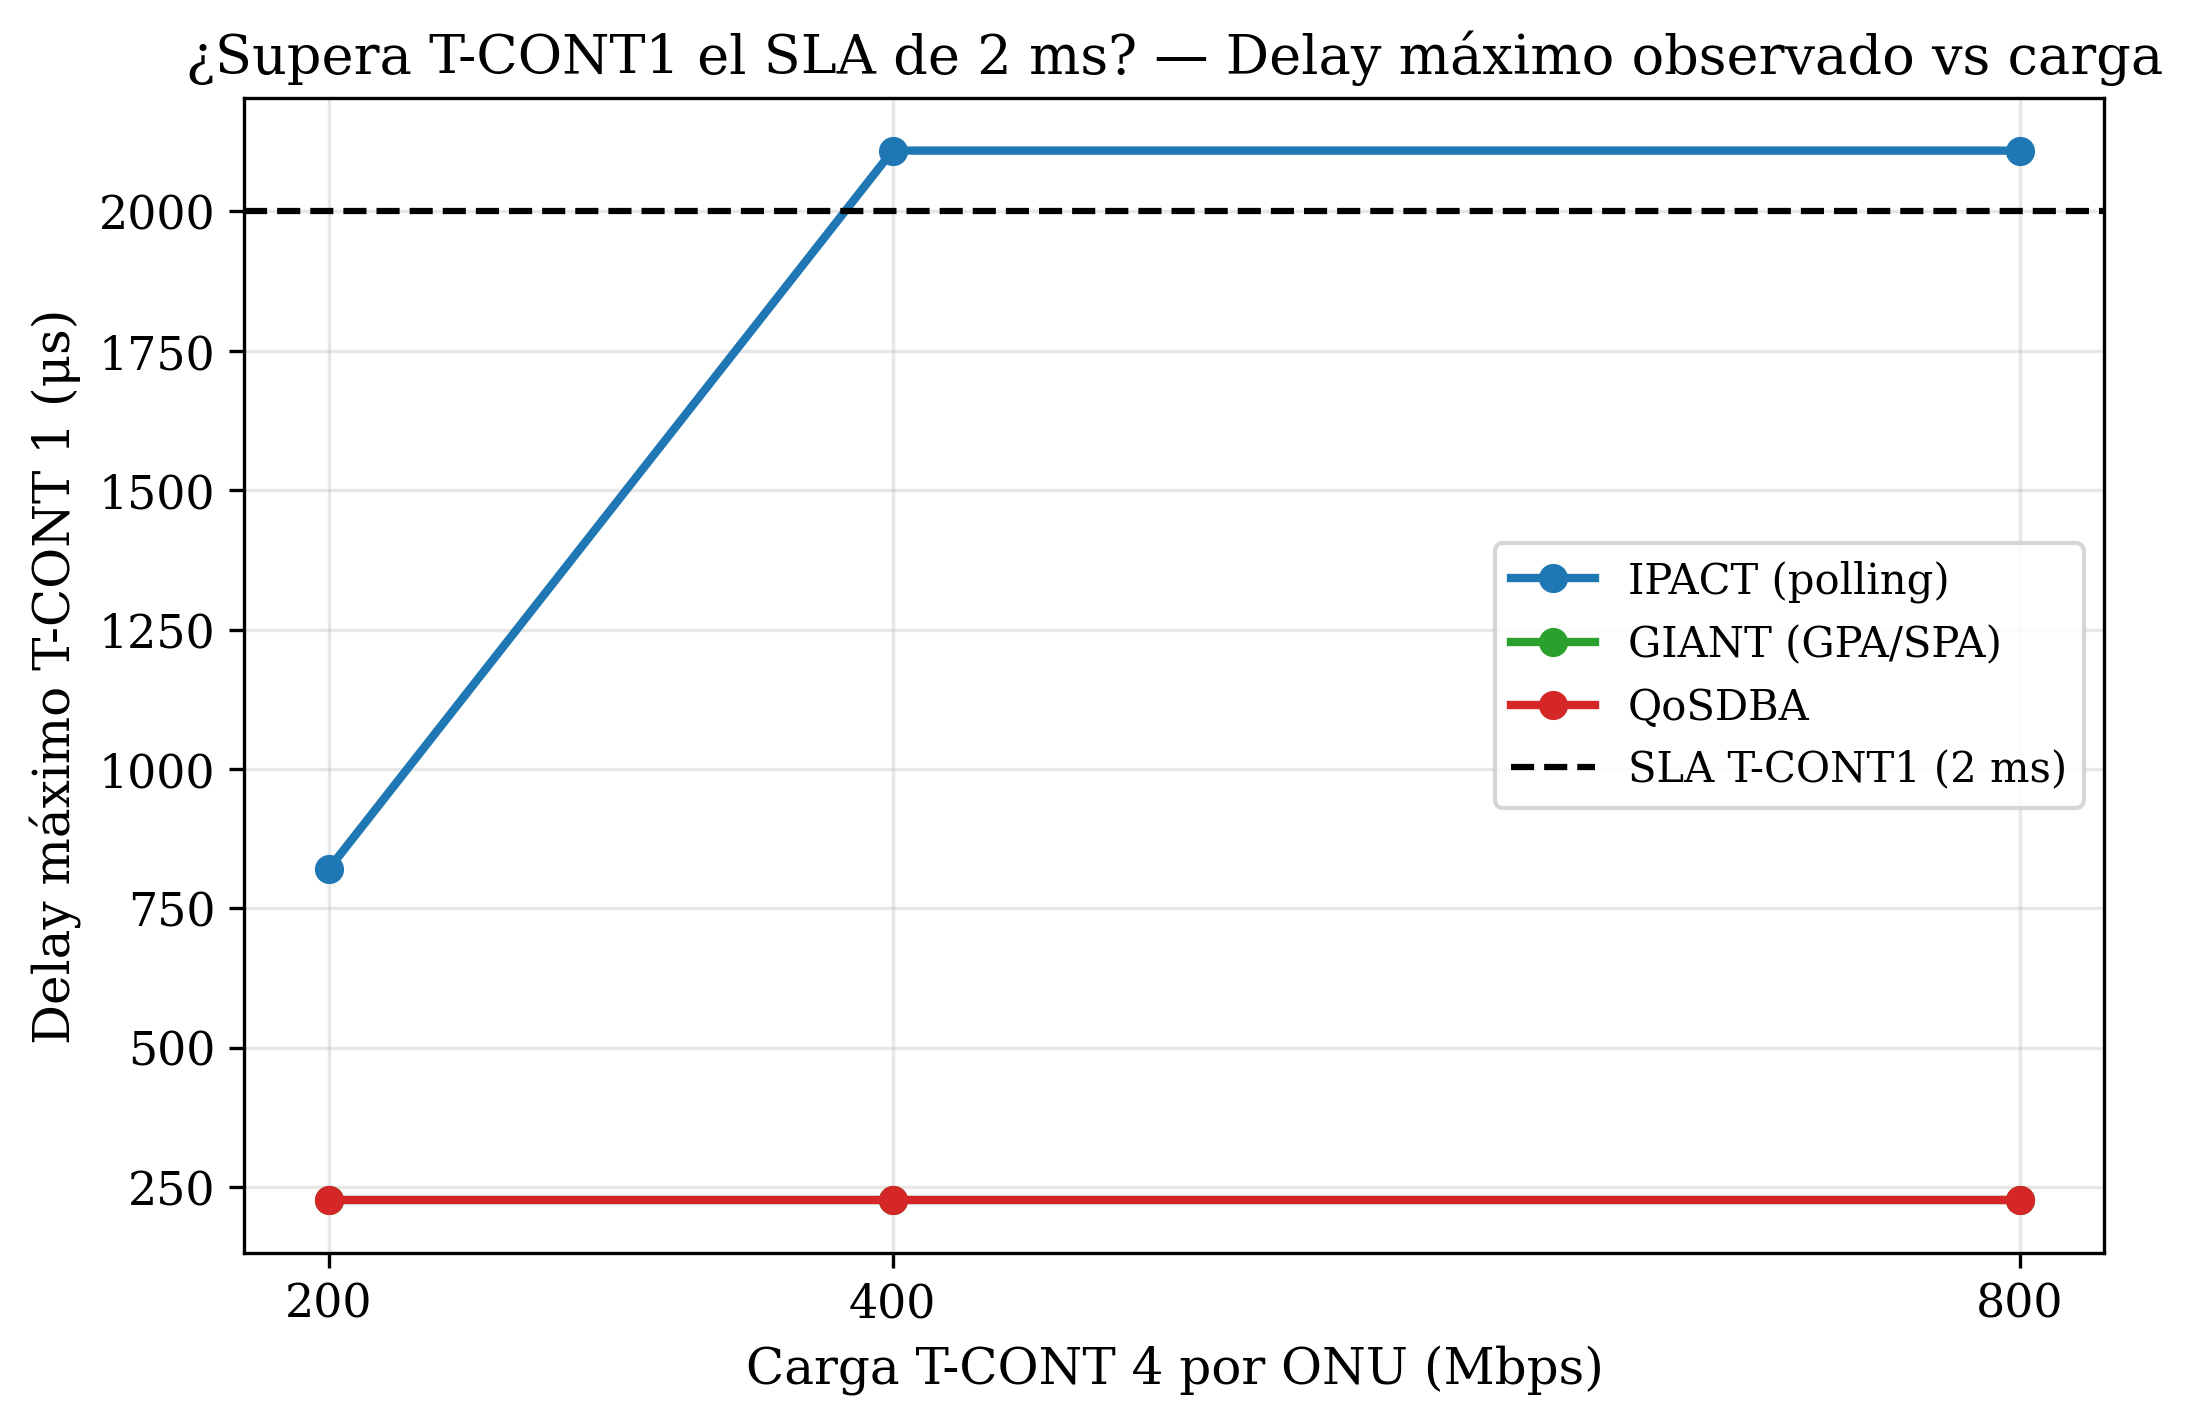
\includegraphics[width=\columnwidth]{max_delay_tcont1_vs_load.png}
\caption{Delay máximo de T-CONT1 vs. carga, con cota de SLA (2 ms).}
\label{fig:delay}
\end{figure}

\begin{figure*}[t]
\centering
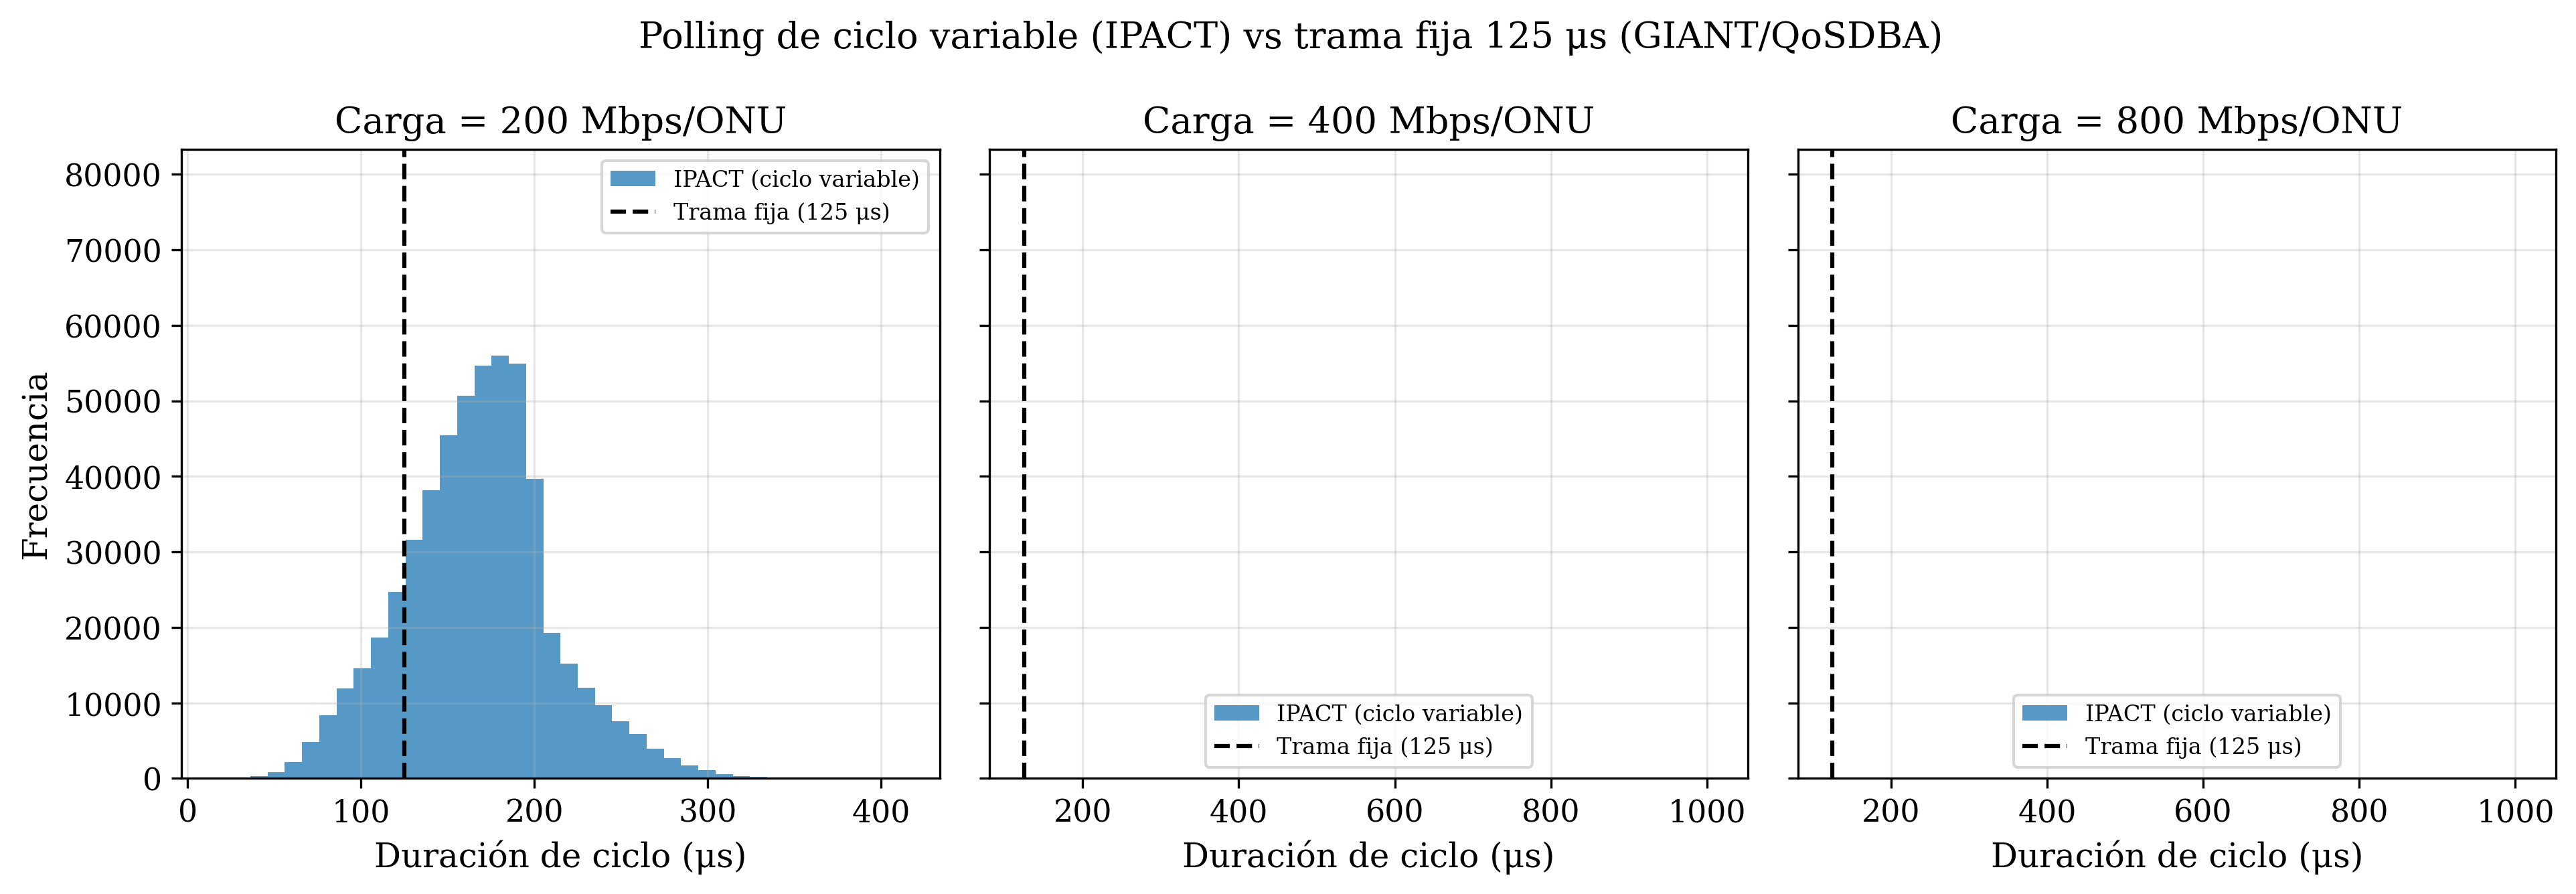
\includegraphics[width=0.85\textwidth]{cycle_time_distribution.png}
\caption{Distribución del ciclo de polling de IPACT vs. trama fija de 125 $\mu$s (GIANT/QoSDBA), por carga.}
\label{fig:cycle}
\end{figure*}

\begin{figure}[h]
\centering

\includegraphics[width=\columnwidth]{throughput_vs_load.png}
\caption{Throughput agregado vs. carga, con referencia de capacidad.}
\label{fig:throughput}
\end{figure}

\subsection{Análisis estadístico}

Cada escenario se corrió con 10 réplicas independientes e idénticamente
distribuidas (semillas 6767--6776), descartando 1 s de \emph{warmup} de
10 s simulados, siguiendo a Law y Kelton \cite{lawkelton}. El intervalo
de confianza al 95\% se calculó como $\bar{y} \pm 1.96\,s/\sqrt{10}$
sobre las 10 réplicas. Como ejemplo de error relativo
(IC95\%/media): la latencia media de T-CONT1 bajo IPACT a 400 Mbps/ONU es
$1613.08 \pm 0.33\,\mu$s, un error relativo de apenas 0.02\%, lo que
indica baja variabilidad entre réplicas para esa métrica. En los caminos
puramente deterministas (T-CONT1 bajo GIANT/QoSDBA, sin uso de números
aleatorios) el IC95\% es exactamente 0, ya que las 10 réplicas producen
resultados idénticos bit a bit.

\section{Conclusiones}
\label{sec:conclusiones}

El proyecto cumplió los objetivos planteados tras el pivote a Fase 3:
implementar un simulador propio (sin frameworks) de XG-PON1, comparar
tres algoritmos DBA bajo una métrica de SLA explícita, y validar el
modelo contra cotas teóricas cerradas. El hallazgo central es que
cumplir el SLA de voz no es automático: depende de cómo decide
el algoritmo de DBA. Reservar ancho de banda sin condiciones (GIANT,
QoSDBA) garantiza el SLA de voz en todo escenario probado, mientras que
asignar según un reporte de demanda (IPACT) puede fallar justo cuando más
se necesita, bajo carga alta y con un reporte desactualizado, aunque a
cambio logra mayor eficiencia agregada que el reparto proporcional de
QoSDBA.

Como lección aprendida, el equipo destaca que declarar explícitamente las
simplificaciones del modelo (8 ONUs idénticas, IPACT como adaptación de
EPON, semántica propia de los contadores de GIANT) resultó más valioso
para la evaluación que intentar modelar cada detalle del estándar, ya que
permitió aislar con claridad la variable de interés.

Como trabajo futuro se propone: introducir \emph{ranging} dinámico
(ONUs a distancias distintas, RTT variable en vez de fijo); permitir
múltiples T-CONTs del mismo tipo por ONU, en vez de la correspondencia
1:1 actual; hacer que GIANT opere a nivel de T-CONT en vez de a nivel de
ONU, como en una implementación real; y evaluar ONUs heterogéneas con
distintos perfiles de tráfico simultáneos.

\begin{thebibliography}{9}

\bibitem{itu987-1}
ITU-T Recommendation G.987.1, ``10-Gigabit-capable passive optical
networks (XG-PON): General requirements,'' International
Telecommunication Union, 2016.

\bibitem{itu987-2}
ITU-T Recommendation G.987.2, ``10-Gigabit-capable passive optical
networks (XG-PON): Physical media dependent (PMD) layer specification,''
International Telecommunication Union, 2016.

\bibitem{itu987-3}
ITU-T Recommendation G.987.3, ``10-Gigabit-capable passive optical
networks (XG-PON): Transmission convergence (TC) layer specification,''
International Telecommunication Union, 2014.

\bibitem{itu984-3}
ITU-T Recommendation G.984.3, ``Gigabit-capable passive optical networks
(GPON): Transmission convergence layer specification,'' International
Telecommunication Union, 2014.

\bibitem{kramer2002}
G. Kramer, B. Mukherjee, and G. Pesavento, ``IPACT: a dynamic protocol
for an Ethernet PON (EPON),'' \emph{IEEE Communications Magazine},
vol.~40, no.~2, pp.~74--80, 2002.

\bibitem{leland94}
W. E. Leland, M. S. Taqqu, W. Willinger, and D. V. Wilson, ``On the
self-similar nature of Ethernet traffic,'' \emph{IEEE/ACM Transactions
on Networking}, vol.~2, no.~1, pp.~1--15, 1994.

\bibitem{lawkelton}
A. M. Law and W. D. Kelton, \emph{Simulation Modeling and Analysis},
3rd ed. New York: McGraw-Hill, 2000.

\bibitem{giant}
Material de cátedra, TEL-341 Simulación de Redes, Universidad Técnica
Federico Santa María, 2026 (esquema GPA/SPA de GIANT, contadores de
\emph{service interval} SImax/SImin).

\end{thebibliography}

\end{document}
